% !TEX root = Main.tex

\appendix
\appendixpage
\addappheadtotoc
%\section{Animation of \nth{9} mode}
%\begin{center}
%  \animategraphics[autoplay,loop,width=\textwidth]{60}{VNL/Frames/frame}{1}{60}
%\end{center}
\section{Mechanics and dynamics of a simple system containing two atoms}\label{Simplemec}
To describe the dynamics of the system one must decompose the system into simpler elements in order to understand what happens for the system as a whole. Basically we want to describe the displacements each atom makes and then sum it up to some bigger form of system. The basis of a system containing only two atoms can be described a mass-spring system where each atom has a mass and where the \textit{atomic interaction potential} works as the spring in between each atom. The interaction potential that we will be working with is called the \textit{Lennard-Jones Potential}\text{\cite[eq.1.3]{Cleland2003}}. The potential in its simplified an general form is given by \begin{equation}
    \phi(r)=-\dfrac{A}{r^{6}}+\dfrac{B}{r^{12}}\label{LJPot}
\end{equation} where $A$ is the strength of the attractive interaction , $B$ is the strength of the repulsive interaction and $r$ is the spacing between the atoms.
The potential can be derived from the force between the atoms as the force is the derivative of the negative potential energy with respect to the atom spacing $r$\text{\cite[eq.1.1]{Cleland2003}}.\begin{equation}
    f(r)\equiv -\dfrac{\text{d}\phi}{\text{d}r}
\end{equation} However it is more convenient to work with the potential instead of the force. \\
The system is in a relaxed state when the distance between the atoms is equal to the \textit{equilibrium distance} $r=r_{0}$. The equilibrium distance\text{\cite[p.3]{Cleland2003}} is given by \begin{equation}
    r_{0}=\left(\dfrac{2B}{A}\right)^{\dfrac{1}{6}}\label{eqdist}
\end{equation} Inserting \eqref{eqdist} in \eqref{LJPot} gives the minimum potential energy \begin{equation}
    \phi(r_{0})=-\dfrac{A^{2}}{4B}
\end{equation}When we work with larger systems we want the system to be relaxed i.e. in equilibrium first. However, for such systems it is not always the case hence why it must be relaxed with the required relaxation energy before we can apply external forces on it. Now that the small system has been described in its equilibrium state. We want to know what happens when we displace the atoms from their equilibrium position, that is to exert an external force on the atoms. As it is with all masses within classic mechanical theory, the atoms will start to oscillate around their equilibrium position. Therefore a \textit{harmonic potential approximation} is needed to describe the energy associated with such a displacement. This approximation only works for small displacements from equilibrium i.e. small external forces. This is because the approximation is made by using a \textit{Taylor series} expansion\text{\cite[eq.1.5]{Cleland2003}} where only the first and second order terms are kept hence the approximation fails the further you get away from the equilibrium position. The expansion of the potential is given by
\begin{align}
    & \phi(r)=\phi(r_{0})+\left\dfrac{\text{d}\phi}{\text{d}r} \right|_{r_{0}}(r-r_{0})+\nonumber\\ & \left\dfrac{1}{2!}\dfrac{\text{d}^{2}\phi}{\text{d}r^{2}}\right|_{r_{0}} (r-r_{0})^{2}+\nonumber\\ & \dfrac{1}{3!}\left\dfrac{\text{d}^{3}\phi}{\text{d}r^{3}}\right|_{r_{0}}(r-r_{0})^{3}+...
\end{align}Where the term $\left\dfrac{\text{d}\phi}{\text{d}r} \right|_{r_{0}}$ equals 0 at equilibrium position. Dropping the higher order terms the series becomes the \textit{harmonic potential approximation}\text{\cite[eq.1.5]{Cleland2003}}\begin{equation}
    \phi(r)\approx \phi(r_{0})+\left\dfrac{1}{2}\dfrac{\text{d}^{2}\phi}{\text{d}r^{2}}\right|_{r_{0}}(r-r_{0})^{2}\label{Harmapprox}
\end{equation}It can be seen that the potential energy depends on the displacement from equilibrium squared. When the atoms are in the presence of an external force, that is when they are displaced from equilibrium. The total potential energy\text{\cite[p.4]{Cleland2003}} becomes $U_{tot}=\phi(r)+\phi_{ext}(r)$, where $\phi_{ext}(r)=-f_{ext}r$. When a constant external force acts on the system, the point of equilibrium moves to a new location. At the location, the derivative of the total potential energy with respect to the displacement is zero
$\dfrac{\text{d}U_{tot}}{\text{d}r}=0$. Working on with this expression and using the result in \eqref{Harmapprox} the total energy in the point of the new equilibrium can described as\begin{align}
    & \dfrac{\text{d}U_{tot}}{\text{d}r}=\dfrac{\text{d}\phi(r)}{\text{d}r}+\dfrac{\text{d}\phi_{ext}(r)}{\text{d}r}=0\nonumber\\
    & \dfrac{\text{d}}{\text{d}r}\left(\phi(r_{0})+\dfrac{1}{2}\left\dfrac{\text{d}^{2}\phi(r)}{\text{d}r^{2}}\right|_{r_{0}}(r-r_{0})^{2}\right)-\nonumber\\ & \dfrac{\text{d}}{\text{d}r}f_{ext}r=0\nonumber\\
    &\dfrac{\text{d}}{\text{d}r}\left(\dfrac{1}{2}\left\dfrac{\text{d}^{2}\phi(r)}{\text{d}r^{2}}\right|_{r_{0}}(r-r_{0})^{2}\right)-f_{ext}=0
    \end{align}The square of the displacement gives the three terms $r^{2}-2r_{0}r+r_{0}^{2}$ that only leaves $2r-2r_{0}$ when derived with respect to $r$. This leaves\begin{align}
   & \dfrac{1}{2}\left\dfrac{\text{d}^{2}\phi(r)}{\text{d}r^{2}}\right|_{r_{0}}(2r-2r_{0})-f_{ext} =0\nonumber\\
   & \left\dfrac{\text{d}^{2}\phi(r)}{\text{d}r^{2}}\right|_{r_{0}}(r-r_{0}) =f_{ext}\nonumber\\
   & r-r_{0} =\dfrac{1}{\text{d}^{2}\phi(r)/\text{d}r^{2}}f_{ext}\label{hooke}
    \end{align}If the  displacement is defined as $u\equiv r-r_{0}$ we can see that \eqref{hooke} is an equivalent to Hooke's Law.\begin{equation}
        u\equiv r-r_{0}=\dfrac{1}{\text{d}^{2}\phi(r)/\text{d}r^{2}}f_{ext}=\dfrac{1}{k}f_{ext}
    \end{equation}Where $k=\dfrac{\text{d}^{2}\phi(r)}{\text{d}r^{2}}$ acts as the spring constant. This last result emphasises that the system of two atoms can be viewed as a mass-spring system.\\
    \eqref{hooke} can also be used to find the equation of motion. As the force equals mass times acceleration the equation must satisfy\begin{equation}
        f_{ext}=\left\dfrac{\text{d}^{2}\phi(r)}{\text{d}r^{2}}\right|_{r_{0}}u=ma=m\dfrac{\text{d}^2}{\text{d}t^2}u
    \end{equation}For the specific case of the two atoms the equation becomes\begin{equation}
        \mu \dfrac{\text{d}^2}{\text{d}t^{2}}u=-\left\dfrac{\text{d}^{2}\phi(r)}{\text{d}r^{2}}\right|_{r_{0}}u\label{eqmotion}
    \end{equation}Where $\mu$ is the reduced mass of the two atoms $\dfrac{1}{\mu}=\dfrac{1}{m_{1}}+\dfrac{1}{m_{2}}$ and the sign in front of the right side of \eqref{eqmotion} is indicating that the force is the restoring force opposing the external force $f_{ext}$. The normal mode solution\text{\cite[eq.1.17]{Cleland2003}} to this equation is\begin{equation}
        u(t)=u_{0}\text{cos}(\omega_{0}t+\varphi)=\text{Re}\left(u_{0}e^{-i\omega_{0}t}\right)
    \end{equation} and the resonance frequency $\omega_{0}$\text{\cite[eq.1.18]{Cleland2003}} is given by\begin{equation}
        \omega_{0}=\sqrt{\dfrac{1}{\mu}\dfrac{\text{d}^2\phi}{\text{d}r^{2}}}=\sqrt{\dfrac{k}{\mu}}
    \end{equation} This concludes the example of a system of two atoms. 
    The next step is to scale up this theory to two and three dimensions.

\section{Boundary Conditions in Two Dimensions}\label{BC}
When describing the motion of the atoms in the lattice as well as the forces acting upon them, some boundary conditions must be defined. Because the system is very large compared to the characteristic wavelength in the displacement field, periodic boundary conditions (PBC) work well. The actual boundaries as well as the specific normal modes are not of significant importance due the same fact of size difference in the system vs. the characteristic wavelength. \\
An intuitive approach to imagining PBC is to take the plane of the system and fold it in to at torus. All the four edges has now been put together pairwise. This means that any force acting on one atom which causes some form of motion is now translated on to the atom next to it.\\
For an arbitrary system in two dimensions of size $X$ (side lenght) and with atomic spacing $r_{0}$, each axis has $\mathcal{N}=\dfrac{X}{r_{0}}$ atoms. The total amount of atoms in the sheet naturally becomes $N=\mathcal{N}^{2}$. The Bloch wavevector can be described as
\begin{equation}
     \mathbf{q}=(q_{x},q_{y})
\end{equation}
where
\begin{equation}
     (q_{x},q_{y})=\dfrac{2\pi}{X}(m,n)
\end{equation}
Here $m,n$ are integers in the interval $-\dfrac{\mathcal{N}}{2}, +\dfrac{\mathcal{N}}{2}$. The range of $q_{x},q_{y}$ becomes $-\dfrac{\pi}{r_{0}},+\dfrac{\pi}{r_{0}}$.\\
In the specific case of this study we work with a fixed boundary, more specific, a clamped boundary which means that no bending is allowed in the plane. A clamped boundary results in the need for numerical approximations in calculations of the dynamics. As the tools used for calculations are on a"per atom" atom basis, there wont be any need for finite-element models nor any partial differential equations solver (PDE).

\section{Plots of RMS-values with varying mode numbers}\label{PLOTZ}

\begin{figure}
    \centering
    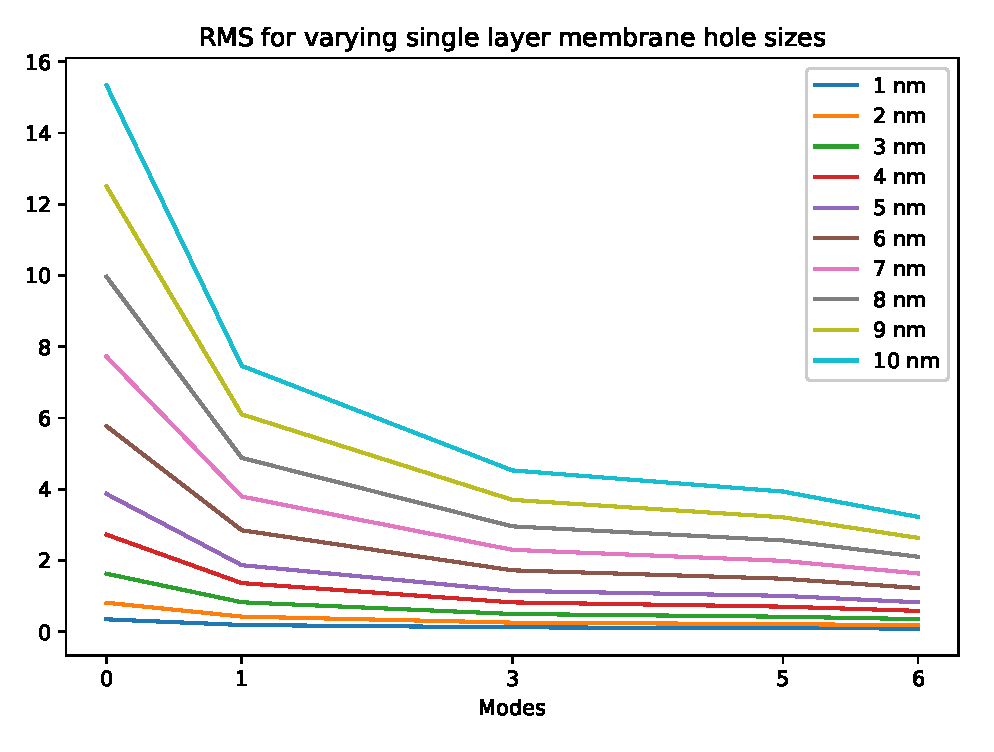
\includegraphics{Figures/RMSvsSize.eps}
    \caption{Figure showing how the RMS decreases as the modes increase. The y-axis are the RMS values for the 10 different membrane sizes as a function of the modes.}
    \label{plot1}
\end{figure}



% \section{Code Compendium}\label{CoCo}
% \subsection{NanoSheetCreator.py}
% \inputminted[python3=true,bgcolor=Black,linenos=true]{python}{VNL/PythonScripts/Scripts/NanoSheetCreator.py}
% \subsection{NanoMembraneCreator.py}
% \inputminted[python3=true,bgcolor=Black,linenos=true]{python}{VNL/PythonScripts/Scripts/NanoMembraneCreator.py}
% \subsection{00\_FixConstraints.py}
% \inputminted[python3=true,bgcolor=Black,linenos=true]{python}{VNL/PythonScripts/Scripts/00_FixConstraints.py}
% \subsection{01\_RelaxSheet.py}
% \inputminted[python3=true,bgcolor=Black,linenos=true]{python}{VNL/PythonScripts/Scripts/01_RelaxSheet.py}
% \subsection{01\_LennardJonesRelax.py}
% \inputminted[python3=true,bgcolor=Black,linenos=true]{python}{VNL/PythonScripts/Scripts/01_LennardJonesRelax.py}
% \subsection{02\_DynamicalMatrix.py}
% \inputminted[python3=true,bgcolor=Black,linenos=true]{python}{VNL/PythonScripts/Scripts/02_DynamicalMatrix.py}
% \subsection{03\_SheetVibrations.py}
% \inputminted[python3=true,bgcolor=Black,linenos=true]{python}{VNL/PythonScripts/Scripts/03_SheetVibrations.py}
% \subsection{DataExtract.py}
% \inputminted[python3=true,bgcolor=Black,linenos=true]{python}{VNL/PythonScripts/Scripts/DataExtract.py}
% \subsection{MyAnalysisFunctions.py}
% \inputminted[python3=true,bgcolor=Black,linenos=true]{python}{VNL/PythonScripts/Scripts/MyAnalysisFunctions.py}
% \subsection{ProjectionPlotter.py}
% \inputminted[python3=true,bgcolor=Black,linenos=true]{python}{VNL/PythonScripts/Scripts/ProjectionPlotter.py}
% \subsection{ZetaPlotter.py}
% \inputminted[python3=true,bgcolor=Black,linenos=true]{python}{VNL/PythonScripts/Scripts/ZetaPlotter.py}
% \subsection{2DdataExtract.py}
% \inputminted[python3=true,bgcolor=Black,linenos=true]{python}{VNL/PythonScripts/Scripts/2DdataExtract.py}
% \subsection{2DmodePlotter.py}
% \inputminted[python3=true,bgcolor=Black,linenos=true]{python}{VNL/PythonScripts/Scripts/2DmodePlotter.py}